\documentclass[12pt,a4paper]{article}
\usepackage{ctex}
\usepackage{amsmath,amscd,amsbsy,amssymb,latexsym,url,bm,amsthm}
\usepackage{epsfig,graphicx,subfigure}
\usepackage{enumitem,balance}
\usepackage{wrapfig}
\usepackage{mathrsfs,euscript}
\usepackage[usenames]{xcolor}
\usepackage{hyperref}
\usepackage[vlined,ruled,commentsnumbered,linesnumbered]{algorithm2e}

\newtheorem{theorem}{Theorem}
\newtheorem{lemma}[theorem]{Lemma}
\newtheorem{proposition}[theorem]{Proposition}
\newtheorem{corollary}[theorem]{Corollary}
\newtheorem{exercise}{Exercise}
\newtheorem*{solution}{Solution}
\newtheorem{definition}{Definition}
\theoremstyle{definition}


%\numberwithin{equation}{section}
%\numberwithin{figure}{section}

\renewcommand{\thefootnote}{\fnsymbol{footnote}}

\newcommand{\postscript}[2]
 {\setlength{\epsfxsize}{#2\hsize}
  \centerline{\epsfbox{#1}}}

\renewcommand{\baselinestretch}{1.0}

\setlength{\oddsidemargin}{-0.365in}
\setlength{\evensidemargin}{-0.365in}
\setlength{\topmargin}{-0.3in}
\setlength{\headheight}{0in}
\setlength{\headsep}{0in}
\setlength{\textheight}{10.1in}
\setlength{\textwidth}{7in}
\makeatletter \renewenvironment{proof}[1][Proof] {\par\pushQED{\qed}\normalfont\topsep6\p@\@plus6\p@\relax\trivlist\item[\hskip\labelsep\bfseries#1\@addpunct{.}]\ignorespaces}{\popQED\endtrivlist\@endpefalse} \makeatother
\makeatletter
\renewenvironment{solution}[1][Solution] {\par\pushQED{\qed}\normalfont\topsep6\p@\@plus6\p@\relax\trivlist\item[\hskip\labelsep\bfseries#1\@addpunct{.}]\ignorespaces}{\popQED\endtrivlist\@endpefalse} \makeatother



\begin{document}
\noindent

%========================================================================
\noindent\framebox[\linewidth]{\shortstack[c]{
\Large{\textbf{Exercise Sheet 13}}\vspace{1mm}\\
Discrete Mathematics by Hongfei Fu, 2022.11.10}}

\begin{center}
	\footnotesize{\color{black} \quad Name:\_\_\_\_\_\_\_\_\_  \quad Student ID:\_\_\_\_\_\_\_\_\_ \quad Class: \_\_\_\_\_\_\_\_\_\_\_\_} \\

\end{center}

\begin{enumerate}
\item ([R], Page 689, Exercise 2(a)(b)(d)) 
Does each of these lists of vertices form a path in the following graph? Which paths are simple? Which are circuits? What are the lengths of those that are paths?\\
$a) a, b, e, c, b$\\
$b) a, d, a, d, a$\\
$d) a, b, e, c, b, d, a$\\
\includegraphics*[scale=0.7]{2@p689.png}

\textbf{Answer Area:}
\vspace{8cm}

\item ([R], Page 689, 6) 
How many connected components does each of the graphs in Exercises 3-5 have? For each graph find each of its connected components.\\
\includegraphics*[scale=0.5]{6@p689.png}

\textbf{Answer Area:}
\vspace{8cm}
\clearpage

\item ([R], Page 690, 14(a)(b)(c)) Find the strongly connected components of each of these graphs.\\
\includegraphics*[scale=0.7]{14@p690.png}

\textbf{Answer Area:}
\vspace{6cm}

\item ([R], Page 692, Exercise 63, \textbf{2pt})  Show that a simple graph $G$ is bipartite if and only if it has no circuits with an odd number of edges.

\textbf{Answer Area:}
\vspace{6cm}


\item (Additional Homework, \textbf{3pt})  

{\bf Matriods.} A finite {\color{red} matroid} is an ordered pair $({\color{blue} E}, {\color{blue} \mathcal{I}})$, where $\color{blue} E$ is a finite set and ${\color{blue} \mathcal{I}}\subseteq 2^{\color{blue} E}$ is a collection of subsets of $\color{blue} E$ such that 
\begin{itemize}
\item $\emptyset\in \mathcal{I}$, and 
\item for any sets $A\subseteq B\subseteq {\color{blue} E}$, if $B\in {\color{blue} \mathcal{I}}$ then $A\in {\color{blue} \mathcal{I}}$, and 
\item for any sets $A, B\in {\color{blue} \mathcal{I}}$, if $|A|<|B|$ then there exists $x\in B\backslash A$ such that $A\cup \{x\}\in {\color{blue} \mathcal{I}}$.   
\end{itemize}

{\bf Disjoint Paths.}
Let ${\color{blue} G}=({\color{blue} V}, {\color{blue} E})$ be a(n undirected) simple graph.
Given a path $\rho=x_0, e_1, \dots, x_{n-1}, e_{n}, x_n$ in $\color{blue} G$, we denote by $\mbox{\sl \color{blue} Edges}(\rho)$ the set of all edges appearing in $\rho$, i.e., 
${\mbox{\sl \color{blue} Edges}}(\rho):=\{e_1, \dots, e_n\}$. 
We say that two paths $\rho, \rho'$ in $\color{blue} G$ are {\color{red} disjoint} if $\mbox{\sl \color{blue} Edges}(\rho)\cap \mbox{\sl \color{blue} Edges}(\rho')=\emptyset$. 

{\bf Independent Sets of Vertices.}
Let ${\color{blue} G}=({\color{blue} V}, {\color{blue} E})$ be a(n undirected) connected simple graph such that $|{\color{blue} V}|\ge 2$.
We assume a designated vertex $\color{blue} v^*$ called the {\color{orange} source} vertex.    
A set $U\subseteq {\color{blue} V}\backslash\{{\color{blue} v^*}\}$ of vertices is called {\color{red} independent} if $U=\{u_1, \dots, u_k\}$ ($k$ can be zero) and there are $k$ pairwise-disjoint paths $\rho_1, \dots, \rho_k$ 
such that each path $\rho_i$ connects $v^*$ and $u_i$ (as endpoints).
Define $\color{red} \mathcal{I}$ to be the set of all independent sets of vertices.  

\textbf{Show} that $({\color{red} V}\backslash\{v^*\}, {\color{red} \mathcal{I}})$ is a finite matroid. 

\textbf{Hint:} The most difficult part is to prove that $({\color{red} V}\backslash\{v^*\}, {\color{red} \mathcal{I}})$ satisfies the third condition in the definition of finite matroids. Given two sets of vertices $A,B\in {\color{red} \mathcal{I}}$, we iteratively construct a sequence of sets of vertices $C_0, C_1, \dots, C_k$ such that the final set $C_k$ of the sequence satisfies that $A\subseteq C_k$ and $|C_k|=|B|$. Initially, we set $C_0:=B$. Then at each stage $n$ from $C_n$ to construct $C_{n+1}$, we start with choosing an aribitrary vertex $a\in A\backslash C_n$. If there is a path from $v^*$ to $a$ that is disjoint from all other paths that connects $v^*$ and vertices in $C_n$, then we simply add the vertex $a$ (implicitly with its path) into $C_n$ and kick out an arbitrary vertex from $C_n\backslash A$. Otherwise, a main phenomenon is that the path $\rho$ from $v^*$ to $a$ conflicts with some path $\rho'$ from $v^*$ to some $b\in B$. Let $e$ be the last overlapping edge on $\rho$ that conflicts with some $\rho''$ as stated above. Then we construct a path from $v^*$ to $a$ by first following $\rho''$ until $e$ and $\rho$ after $e$. By iterating the progress from $C_n$ to $C_{n+1}$, the overlapping edges $e$ can only move closer to $v^*$ as the paths to vertices in $A$ are guaranteed to be disjoint. Since, we cannot get infinitely closer to $v^*$, the construction of the sequence $C_0,C_1,\dots$ must end at some $C_k$, and at the end we must have that $C_k$ is independent and $A\subseteq C_k$. 

\textbf{Answer Area:}
\vspace{10cm}
~\\
\vspace{10cm}

\item (Additional Homework, \textbf{5pt})

{\bf Augmenting Paths.} Let $G=(V, E)$ be a bipartite graph with bipartition $(V_1,V_2)$. 
An \emph{augmenting path} w.r.t a matching $M$ in $G$ is a simple path with distinct vertices that (i) starts with some edge from $E\backslash M$, (ii) alternately follows edges from $M$ and $E\backslash M$, and (iii) ends at some edge from $E\backslash M$. For example, in Figure~\ref{augmenting}, we have that a path $a,b,c,d,e,f$ of $G$ is an augmenting path with respect to the matching $M=\{ed, bc, gh\}$ (we write $uv$ as a short-hand for the edge $\{u,v\}$). The path is augmenting since it can enlarge the matching if we exchange $bc, de$ with $ab, cd, ef$. 

\begin{figure}[h]
\centering
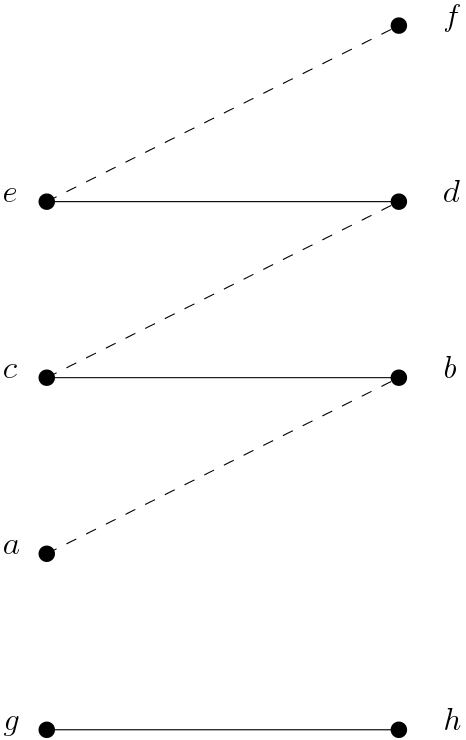
\includegraphics[scale=0.5]{augmenting}
\caption{An Augmenting Path}
\label{augmenting}
\end{figure}

To be more detailed, an \emph{augmenting path} with respect to a matching $M$ in $G$ is a simple path of distinct vertices $u_1,v_1,\dots, u_n,v_n$ in $G$ such that:
\begin{enumerate}
\item $u_i\in V_1$ and $v_i\in V_2$ for all $1\le i\le n$, and 
\item $u_iv_i$'s ($1\le i\le n$) and $u_iv_{i-1}$'s  ($2\le i\le n$) are edges of $G$, and 
\item both $u_1$ and $v_n$ are unmatched in $M$, and 
\item the edges $u_2v_1, \dots, u_nv_{n-1}$ fall in $M$, and 
\item the edges $u_1v_1, \dots, u_nv_{n}$ are not in $M$. 
\end{enumerate}

Try to solve the following problems.
\begin{itemize}
\item Prove that if a matching $M$ in $G$ is not maximal, then there exists an augmenting path w.r.t $M$. (\textbf{2pt}) 
\item Use augmenting paths to prove Hall's Marriage Theorem. (\textbf{3pt}) \textbf{Hint:} Instead of considering a single augmenting path, one needs to consider \textbf{all} augmenting paths starting from an unmatched vertex.  
\end{itemize}

\textbf{Answer Area:}
\vspace{10cm}

\end{enumerate}
%========================================================================
\end{document}
